% !TEX root =..\main.tex
\section{РАЗРАБОТКА ПРОЕКТА}

        В этой части работы будут описаны конкретные шаги для достижения поставленной задачи.

    \subsection{Настройка окружения}

        Перед началом разработки необходимо настроить окружение и задать структуру проекта. Работа началась с того, что была скачана официальная сборка Godot 4.3 c поддержкой Mono. 
        Существует две версии Godot: с поддержкой Mono и без. Mono позволяет использовать C\# в качестве языка программирования, что является основным требованием к проекту.
        У Godot есть свой редактор кода с подсветкой синтаксиса и автодополнением, однако, он наилучшим образом работает с GDScript -- скриптовым языком, сделанным специально для этого
        движка. Для работы с C\# придется использовать другую среду разработки (IDE), например, Visual Studio или Rider. В данной работе использовалась Visual Studio 2022 Community Edition.
        \begin{figure}[H]
            \centering
            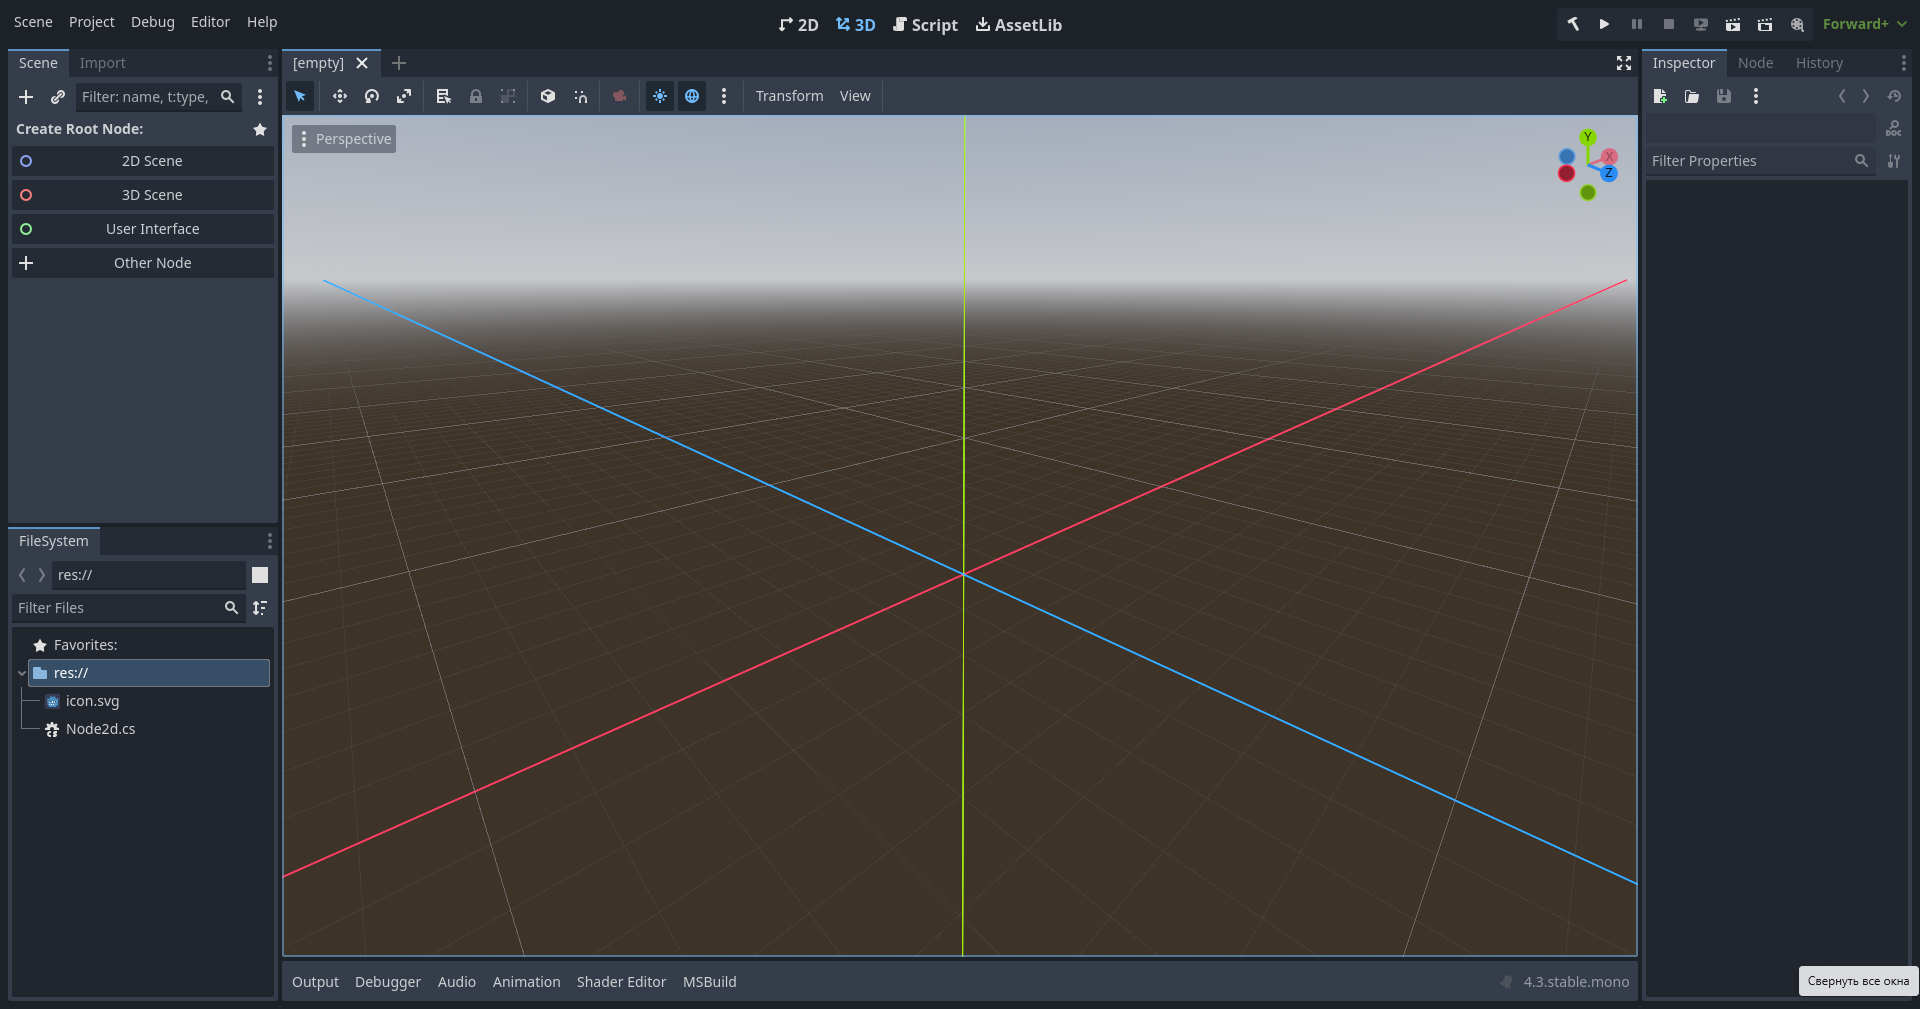
\includegraphics[width=\textwidth]{pictures/godot-editor.png}
            \caption{Редактор Godot}\label{ris2.1}
        \end{figure}
        При запуске и создании проекта нас встречает редактор с пустой 3D-сценой (Рисунок \ref{ris2.1}). Для начала разработки необходим проект C\#, который автоматически создается при
        подключении любого C\#-скрипта к любому узлу. Была создана новая 2D-сцена и корневой узел, к которому затем привязан скрипт. В папке проекта автоматически создадутся .csproj и .sln файлы, с
        которыми уже можно работать в Visual Studio. Поскольку клиент является одним из модулей, вся директория клиента будет являться частью большего по масштабу проекта, в который
        также включены следующие проекты, которые были разработаны в рамках курсовой работы:

        \begin{itemize}
            \item Server -- модуль основного процесса, отвечающего за инициализацию остальных модулей проекта;
            \item SharedObjects -- библиотека классов, содержащая объекты, которые присутствуют в других модулях. Например, класс Gamestate нужен и серверу, и клиенту, чтобы обмениваться информацией об игровом состоянии. Также в этом проекте реализован игровой цикл;
            \item VoiceRecognitionModule -- модуль ASR. В нем находится Vosk -- библиотека для распознавания речи. Цикл этого модуля заключается в том, что он непрерывно считывает голосовой потока с клиента и преобразует его в текст, после чего он пытается интерпретировать команду и отправить ее серверу;
            \item VoiceResponseModule -- модуль TTS, который, на каждый запрос о выполненной команде, синтезирует аудиоответ игроку и отправляет его на клиент.
        \end{itemize}

        Эти модули были написаны на версии .NET 8.0, в то время как C\# проект Godot имеет целевую ОС .NET 6.0, из-за чего возникают проблемы при сборке проекта. Если поменять целевую ОС, то сборка
        проходит успешно.

        Далее нужно подключить отладчик Visual Studio к проекту Godot. Для этого надо создать новый параметр запуска и указать путь для движка.
        
        После всех настроек структура решения изображена на рисунке в \textbf{приложении В}.

        Структура проекта на Citrus, в свою очередь, изображена на рисунке в \textbf{приложении Г}.


        Очевидно преимущество структуры C\#-проекта на Godot, так как она позволяет легко находить нужные файлы и быстро ориентироваться в проекте. Citrus же имеет сложную и громоздкую структуру, 
        которая затрудняет навигацию по проекту. Большинство этих файлов не имеют практического смысла для разработчика, они лишь представляют собой низкоуровневый код и нужны для функционирования 
        движка. 

        В последнюю очередь, стоит определиться со структурой Godot-проекта для комфортной навигации по редактору:
        \begin{itemize}
            \item Assets -- директория с ассетами игр, такими как спрайты, шрифты, звуки и т.д.;
            \item Scenes -- сцены игры. Сцены в Godot -- это отдельные файлы, которые могут содержать узла, скрипты и другие ресурсы. Каждая сцена может быть загружена и использована в игре;
            \item Scripts -- директория со скриптами, содержащие всю логику клиентского приложения. Для каждой сцены скрипты будут помещаться в отдельные директории, поскольку сцены друг от друга никак не зависят и общих ресурсов не имеют;
            \item Shaders -- директория с шейдерами, которые используются для создания эффектов в игре. Шейдеры -- это программы, которые выполняются на графическом процессоре и позволяют создавать визуальные эффекты, не затрагивая логику игры.
        \end{itemize}

        Подводя итог, настройка Godot 4.3 с поддержкой Mono, привязка проекта к Visual Studio 2022 и выстраивание чёткой структуры каталогов 
        создали удобную и прозрачную основу для разработки. 
        Унификация целевого фреймворка на .NET 6.0 позволила собрать все компоненты без конфликтов, а конфиг запуска в IDE обеспечил комфортную отладку C\#-скриптов в среде Godot. 
        В результате проект обрел надёжную и масштабируемую архитектуру, готовую к дальнейшей разработке.


    \subsection{Разработка клиентской части}

        \subsubsection{Система сцен и узлов}
        
        Система сцен и узлов в Godot лежит в основе построения любой игровой логики и интерфейса. Вместо монолитных классов движок предлагает композицию: каждое игровое или вспомогательное 
        звено представлено отдельным узлом (Node), а сцена (Scene) — это файл-контейнер, в котором узлы организованы в древовидную структуру.

        Узел сам по себе ничего не рисует и не обрабатывает ввод, пока не получает <<роли>> через тип. Так, Node2D отвечает за двумерное позиционирование и отрисовку спрайтов, а Control-узлы 
        служат для построения GUI. При необходимости один и тот же узел можно добавить в разные сцены, комбинировать и расширять его функциональность 
        скриптами на C\#.

        Сцена в Godot она может быть сохранена в файл .tscn или .scn и затем <<инстанцирована>> в качестве дочернего элемента в любой 
        другой сцене. Это позволяет организовать вложенные уровни: главная игровая сцена содержит сцену игрового мира, а та, в свою очередь, включает узлы с игровыми объектами.
        Кроме того, Godot поддерживает механизм наследования сцены: на основе базового шаблона можно создать <<наследника>>, добавив или переопределив узлы и скрипты. Это удобно для 
        быстрой генерации вариантов однородных игровых объектов или экранов меню с общим видом.

        Рабочий процесс обычно выглядит так: в редакторе создаётся корневая сцена, где располагаются узлы — камера, фон, интерфейс. Каждый узел настраивается 
        через инспектор: задаются свойства, подключаются скрипты, выставляются приоритеты отрисовки.

        У любого узла можно переопределять методы, отвечающие за логику конкретных событий. Так, метод Ready вызывается единоразово при инициализации узла, Process -- каждый игровой кадр, а Input -- 
        после любого пользовательского ввода. При разработке будут переопределяться именно эти три метода.

        \subsubsection{Глобальные переменные}

        Иногда для реализации игровой логики необходимо передавать информацию между сценами. Для решения этой проблемы в Godot существует концепция глобальных переменных. 
        Глобальные переменные реализуются через механизм singletons, когда пользовательский класс подключается в настройках Godot-проекта и 
        становится доступен из любой сцены по выбранному имени. Через такой singleton удобно хранить состояние о сетевом клиенте информацию об игроке и общие настройки, такие как IP-адрес и порт
        сервера. Доступ к этим переменным прост -- достаточно инициализировать объект в узле и обратиться к полю или методу класса, что избавляет от необходимости передавать данные вручную между 
        узлами и сценами.

        \subsubsection{Сцена главного меню}

        Главное меню -- первая сцена, которая встречает игрока. Через него задаются параметры подключения к серверу и имя игрока. Для его создания используются Control-узлы, представляющие
        различные примитивные элементы интерфейса, такие как ярлык, поле для ввода текста, кнопка, контейнеры для организации этих элементов. Через редактор Godot элементы накладываются друг на
        друга, образуя иерархическую древовидную структуру.

        Для подключения к серверу и началу игрового процесса достаточно трех полей ввода -- для имени игрока, IP-адреса и порта сервера, а также кнопки, по нажатии на которую происходит
        переключение между сценами. У объекта Button есть событие OnButtonPressed, которое вызывается каждый раз при ее нажатии. К этому событию можно привязать метод, который будет
        осуществлять переключение между сценами, предварительно обновляя глобальные переменные, которые пользователь ввел в соответствующие поля ввода:

        \begin{lstlisting}[caption=Реализация логики главного меню]
public override void _Ready()
{
    IPInput = GetNode<TextEdit>("VBoxContainer/IPEdit");
    portInput = GetNode<TextEdit>("VBoxContainer/PortEdit");
    nameInput = GetNode<TextEdit>("VBoxContainer/PlayerNameEdit");

    GetNode<Button>("VBoxContainer/StartButton").Pressed += OnButtonPressed;
}
private void OnButtonPressed()
{
    string playerName = nameInput.Text;
    string ip = IPInput.Text;
    string port = portInput.Text;
    NetworkClient netClient = new NetworkClient();

    Global globals = GetNode<Global>("/root/Global");

    globals.NetworkClient = netClient;
    globals.PlayerName = playerName;
    globals.IPAddress = ip;
    globals.Port = port;
    GetNode<Button>("VBoxContainer/StartButton").Disabled = true;

    GetTree().ChangeSceneToFile("res://Scenes/tile_map.tscn");
}
        \end{lstlisting}

        \subsubsection{Основная сцена}

            В основной сцене реализована непосредственно игровая логика: взаимодействие с сервером, обработка пользовательского ввода и отрисовка игрового состояния,
            присылаемого сервером. В этой сцене находятся следующие узлы:

            \textbf{RootNode}

            RootNode -- корневой узел сцены. Сам по себе не содержит какой-либо игровой логики и не является элементом интерфейса. Данный узел служит связующим звеном между его потомками. 
            
            \textbf{TileMapLayer}

            TileMapLayer представляет собой расширение встроенного в Godot типа узла TileMap, отвечающее за отрисовку и управление одним <<слоем>> тайловой карты. Каждый экземпляр TileMapLayer 
            хранит ссылку на ресурс TileSet, в котором каждому ID тайла сопоставлен спрайт, область коллизий и дополнительные свойства. При инициализации уровня из серверных 
            данных TileMapLayer для каждой клетки вызывает метод SetCell, размещая нужный тайл на сетке с указанным Z-индексом. 
            Отдельные слои (например, база, объекты и подсветка выбранных клеток) создаются как несколько TileMapLayer с разными Z-индексами, что позволяет менять любой слой в 
            реальном времени без перерисовки остальных.

            TileMapLayer поддерживает разные формы тайлов -- квадратную, шестиугольную, изометрическую и квадратную со сдвигом, что существенно облегчит разработку, так как не придется
            реализовывать игровое поле самостоятельно, как было при разработке игры на Citrus.

            Для клиента было реализовано четыре узла TileMapLayer -- слои с рамками клеток, фоном (белый -- свободная клетка, зеленый -- союзный юнит, красный -- вражеский), 
            иконку юнита, а также слой из серых тайлов -- <<туман войны>>

            Для того чтобы создать тайл на слое, нужно подготовить набор текстур, который называется TileSet. В Godot можно быстро создать набор тайлов, загрузив изображение (Рисунок \ref{ris2.4}):
            \begin{figure}[H]
                \centering
                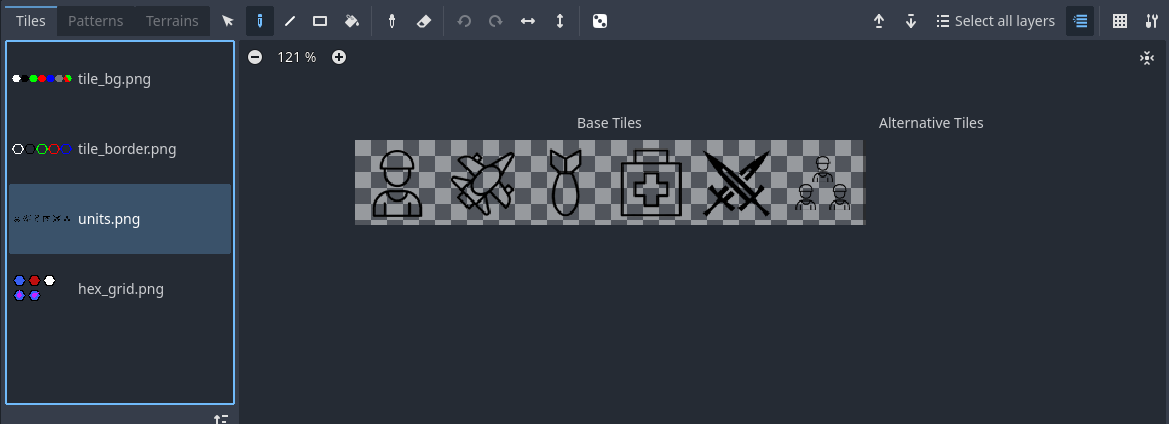
\includegraphics[width=\textwidth]{pictures/godot_tileset.png}
                \caption{Наборы тайлов для слоев TileMapLayer}\label{ris2.4}
            \end{figure}

            При наложении друг на друга, слои образуют понятное для игрока игроков поле, визуализирующее игровое состояние.

            \textbf{CursorHover}

            \textit{CursorHover} -- это узел примитивного типа, к которому привязан скрипт с логикой наведения курсора на TileMapLayer, чтобы отображать ту клетку, на которую
            в текущий момент наведен курсор. Это нужно в первую очередь для удобства навигации игрока по игровой карте. Это реализовывается через смену тайла на слое BorderTileLayer, который
            отвечает за рамку шестиугольной клетки.

            При реализации было учтено несколько важных нюансов: при захвате положения курсора возвращаются координаты относительно окна приложения. То есть,
            если камера будет находиться не в нулевых координатах, то будет выбран не тот тайл, на который наведен курсор. То же самое касается и приближения камеры.

            Для решения этой проблемы нужно учитывать эти параметры камеры при вычислении нужного тайла.

            \begin{lstlisting}[caption=Реализация подсветки тайла]
public override void _Process(double delta)
{
    Viewport viewport = GetViewport();
    Vector2 mousePos = viewport.GetMousePosition();
    mousePos -= viewport.GetWindow().Size / 2; //adjust position by window size
    mousePos /= camera.Zoom; //adjust position by camera zoom
    mousePos += camera.Position; //adjust position by camera coords
    Vector2I tilePos = borderLayer.LocalToMap(mousePos);

    var data = borderLayer.GetCellTileData(tilePos);

    if (data == null)
        return;

    if (currentTile == null || tilePos != currentTile)
    {
        if (currentTile != null && borderLayer.GetCellAtlasCoords(currentTile.Value)[0] != 4)
        {
            OnMouseExitedTile(currentTile.Value);
        }
        currentTile = tilePos;
        if (data != null && borderLayer.GetCellAtlasCoords(tilePos)[0] != 4)
            OnMouseEnteredTile(tilePos);
    }
}

private void OnMouseEnteredTile(Vector2I tileCoords)
{
    borderLayer.SetCell(tileCoords, 1, new Vector2I(2, 0));
}

private void OnMouseExitedTile(Vector2I tileCoords)
{
    borderLayer.SetCell(tileCoords, 1, new Vector2I(1, 0));
}
            \end{lstlisting}


            \textbf{VoiceReceiverNode}

            VoiceReceiverNode -- узел, в котором происходит обработка ввода пользователем звука с микрофона, и в отдельном потоке воспроизводится аудиоответы от сервера. 
            При нажатии на пробел создается канал gRPC и начинается запись голосовой команды. После того как игрок отпускает клавишу, запись останавливается и отправляется в модуль TTS.
            \begin{lstlisting}[caption=Цикл обработки голосового ввода]
public void Update(double delta)
{
    bool isSpacePressed = Input.IsKeyPressed(Key.Space);
    if (_wasSpacePressed && !isSpacePressed)
    {
        waveInEvent.StopRecording();
        Thread.Sleep(100);
        channel?.Dispose();
        callForSendVoice?.Dispose();
        channel = null;
        voiceStreamingClient = null;
        callForSendVoice = null;
    }

    if (!_wasSpacePressed && isSpacePressed)
    {
        channel ??= GrpcChannel.ForAddress("http://localhost:12344");
        voiceStreamingClient ??= new SpeechToCommand.SpeechToCommandClient(channel);
        callForSendVoice ??= voiceStreamingClient.AudioToText();
        waveInEvent.StartRecording();
    }

    _wasSpacePressed = isSpacePressed;
}
            \end{lstlisting}
            
            \textbf{Camera2D}

            Без камеры навигация по игровому полю будет невозможна: его площадь в разы превышает размер окна, и игрок будет видеть лишь малую его долю.
            Для ее реализации Godot предоставляет узел Camera2D, и разработчику лишь остается запрограммировать ее поведение.

            Примитивным вариантом было бы реализовать перемещение камеры при помощи клавиатуры, но в контексте стратегии в реальном времени это весьма неудобно.
            В играх такого жанра навигация по игровой карте традиционно осуществляется при помощи компьютерной мыши. В данном случае будет реализовано перемещение камеры
            при удерживании правой кнопки мыши; при отпускании камера будет фиксировать положение. После того как игрок нажал на кнопку, фиксируются старые координаты
            камеры и положение курсора, и пока игрок не отпустит ее, каждый кадр камера будет смещаться на разницу между текущим и зафиксированным положением курсора,
            тем самым обеспечивая плавное перемещение.

            Также имеет смысл реализовать приближение и отдаление камеры, поскольку карта может быть произвольных масштабов, и для быстрой навигации может быть необходимо
            отдалить камеру.

            Стоит учесть, что, как и в случае с узлом CursorHover, координаты курсора также возвращаются относительно окна. Эта проблема решается аналогичным образом.

            \begin{lstlisting}[caption=Реализация перемещения камеры]
public override void _Input(InputEvent @event)
{
    Viewport viewport = GetViewport();
    Vector2 mousePos = viewport.GetMousePosition();
    mousePos -= viewport.GetWindow().Size / 2; //adjust position by window size
    mousePos += currentCamCoords; //adjust position by camera coords

    if (@event is InputEventMouseButton ev && ev.ButtonIndex == MouseButton.Right)
    {
        if (ev.Pressed)
        {
            dragging = true;
            lastMousePos = mousePos;
        }
        else
        {
            currentCamCoords = Position;
            dragging = false;
        }
    }


    if (@event is InputEventMouseMotion mv && dragging)
    {
        var evPos = mv.Position;
        evPos -= viewport.GetWindow().Size / 2;
        evPos += currentCamCoords;

        var delta = evPos - lastMousePos;
        lastMousePos = evPos;
        Position -= delta/Zoom;
    }

}
            \end{lstlisting}

            \textbf{ClientNode}

            ClientNode -- основной узел сцены, в котором реализован игровой цикл. В нем происходит взаимодействие с сервером и отрисовывается игровое
            состояние. Перед отрисовкой кадра с сервера приходит обновленное состояние. На его основе размещаются тайлы в узлах типа TileMapLayer, причем
            все клетки на поле перекрываются <<туманом войны>>. После размещения юнитов поле очищается от тумана: происходит итерация по всем юнитам игрока,
            и для каждого юнита очищаются клетки в его радиусе обзора.
            
            В этом же узле реализована логика <<активной клетки>>: при нажатии левой кнопки мыши на клетку, она помечается как активная, и в верхнем левом углу
            отображается список юнитов, находящихся в ней, который обновляется динамически. Чтобы достигнуть этого, составляется актуальный список юнитов, 
            присланный от сервера, затем происходит итерация по дочерним узлам элемента интерфейса, отвечающего за отображение юнитов на клетке. Если 
            оказывается, что в окне находится юнит, которого нет в актуальном списке, то этот элемент удаляется. Если оказывается, что кого-то
            не хватает, создается новый элемент и инициализируется. Важно проводить итерацию от последнего дочернего к первому, чтобы в случае удаления
            не нарушалась индексация.
            
        
        \subsubsection{Heads-Up Display (HUD)}

            Одно из преимуществ Godot -- обильное количество встроенных инструментов для верстки сложных элементов пользовательского интерфейса. HUD вынесен в отдельный CanvasLayer, 
            что обеспечивает его отрисовку всегда поверх игровой сцены и независимость от движения камеры. Внутри CanvasLayer строится древовидная структура Control-узлов.
            Были реализованы следующие элементы интерфейса:

            \textbf{CoordsWindow}

            Небольшое окно в левом нижнем углу экрана, отображающее координаты клетки, на которую наведен курсор. Это нужно для удобства навигации и отдачи голосовых команд игроком.
            Данные обновляются на узле CursorHover: перед подсветкой наведенного курсором узла, вызывается метод UpdateCoordsHUD.
            \begin{lstlisting}[caption=обновление интерфейса]
void UpdateHUD(Vector2I coords)
{
    Label xLabel = coordsBox.GetChild<Label>(0);
    Label yLabel = coordsBox.GetChild<Label>(1);

    xLabel.Text = $"X: {coords[0]}";
    yLabel.Text = $"Y: {coords[1]}";
}
            \end{lstlisting}

            \textbf{CellInfoBase и CellInfoContainer}
            
            В процессе игры необходимо знать не только координаты определенной клетки, но и информацию о юнитах, которые на ней находятся. Для этого был создан шаблон
            панели с информацией о юните. Корневым узлом шаблона является PanelContainer -- контейнер с настраиваемым задним фоном (Рисунок \ref{ris2.5}). На него помещены узлы типа VBoxContainer и
            HBoxContainer для корректного размещения узлов, несущих в себе информацию о юните.

            Из информативных узлов присутствуют ярлыки для позывного юнита и значению здоровья в текстовом виде, TextureRect -- область, в которой отрисовывается текстура; в ней будет
            присутствовать иконка юнита. Наконец, для визуального отображения оставшегося здоровья был добавлен TextureProgressBar -- полоса прогресса, на которую можно добавить
            текстуру. Узел этого типа имеет поле Range, в котором можно настраивать <<полноту>> текстуры в виде процентного значения.

            Также в целях отладки была добавлена кнопка типа TextureButton для отдачи команды юнитам в обход голосовому интерфейсу.
            

            \begin{figure}[H]
                \centering
                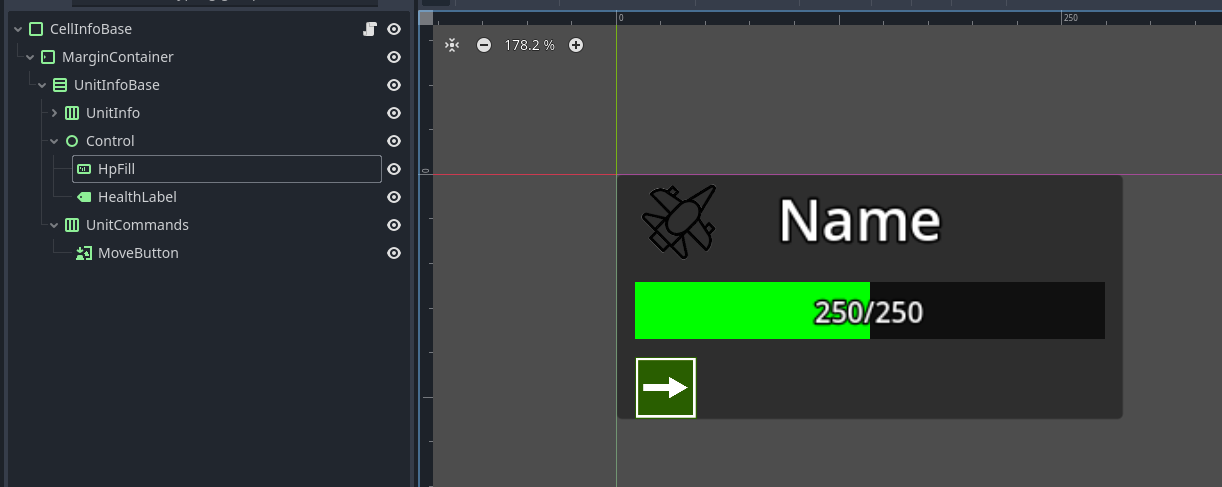
\includegraphics[width=\textwidth]{pictures/cellinfobase.png}
                \caption{Шаблон элемента CellInfo}\label{ris2.5}
            \end{figure}

            Поскольку это шаблон для одного из множества юнитов на поле боя, этот элемент интерфейса нужно сохранить в отдельную сцену, чтобы программно создавать его для каждого юнита.
            Когда на выделенной клетке есть какой-то юнит, происходит <<инстанциация>> сцены, что создает новый узел, повторяющий всю структуру сцены. Этот узел в последствии прикрепляется в
            специальный контейнер с возможностью прокрутки содержимого, становясь его наследником.
            \begin{lstlisting}[caption=Создание экземпляра шаблона]
var unitInfoScene = GD.Load<PackedScene>("res://Scenes/cell_info_base.tscn");
CellInfoBase panel = unitInfoScene.Instantiate<CellInfoBase>();
panel.Setup(selectedCell.Value, currentUnit.Health, currentUnit.MaxHealth, unitId, atlCoords, currentUnit.Nickname);

panel.Handler = (bool toggledOn) =>
{
    OnMoveButtonPressed(panel, toggledOn);
};
panel.MoveButton.Toggled += panel.Handler;

cellInfo.AddChild(panel);
            \end{lstlisting}


    \subsection{Доработка серверной части}

        После завершения разработки клиентской части необходимо было доработать серверную часть. На момент сдачи курсовой работы серверная часть обладала 
        базовым функционалом для работы сетевой составляющей, игрового цикла и голосового интерфейса.

        Для демонстрации возможностей клиента на Godot были добавлены новые геймплейные возможности и устранены недочеты.

        \subsubsection{Единственный юнит на клетке}
        Одним из недочетов было то, что игровое поле было запрограммировано таким образом, что на одной клетке в один момент времени мог находиться лишь 
        один юнит. Когда на нее переходил другой юнит, пока она была занята, информация о расположении этого юнита на клетке пропадала, в то время как сам 
        юнит оставался в игровом состоянии.

        Игровая клетка представляет из себя объект HexCell, являющегося частью объекта HexGrid. В нем было поле CellUnitId -- уникальный идентификатор юнита в 
        игровом мире. Метод UpdateCellUnit заменял значение этой переменной, что приводило к противоречиям в игровом состоянии -- у клетки был один идентификатор
        юнита, а у того, которого сместили -- координаты клетки сместившего его юнита.

        Эта проблема была решена, заменив поле типа int на список уникальных идентификаторов. Для корректной работы также были обновлены методы UpdateCellUnit и
        RemoveCellUnit, которые добавляли и удаляли элемент из списка соответственно.

        \subsubsection{Ошибка в изменении коллекции при итерации}

        При перемещении юнитов сервер периодически завершал работу с ошибкой, которая указывала на изменение коллекции при итерации, в следствие чего 
        происходило обращение по несуществующему индексу. Оказалось, что во время сериализации игрового состояния оно успевало обновиться, из-за чего
        при сериализации списков их размер оказыватся некорректен.

        Решением проблемы была блокировка ресурсов во время итерации с помощью ключевого слова lock. Таким образом, если объект оказывался <<занят>>, 
        другая часть кода, запрашивавшая доступ к этому же ресурсу, ждала освобождение объекта.

        \subsubsection{Сражение юнитов}

        Ключевая механика любой RTS -- сражение на поле боя. До начала работы была лишь реализована механика передвижения. Для задания минимальной
        играбельности необходимо было реализовать сражение хотя бы на базовом уровне.

        Поскольку теперь на одной клетке могут находится несколько юнитов разных игроков, сражения будет обрабатывать HexCell. Далее описан один игровой цикл сражения.
        
        Составляются списки юнитов каждого игрока, затем происходит итерация по этим двум спискам: если юнит может атаковать, он атакует первого попавшегося врага и уходит на перезарядку.
        Если не может, то счетчик перезарядки увеличивается на время, которое прошло с момента прошлого игрового цикла. Если прошло достаточно времени, юнит 
        атакует по той же логике. Если какой-либо из юнитов погибает, их идентификаторы записываются в отдельный массив. После атаки погибшие юниты удаляются из
        игры. Сражение продолжается, пока на клетке не останутся юниты, принадлежащие к одной команде.

        Реализация сражения юнитов продемонстрирована в листинге в \textbf{приложении Д}.
    \subsection{Итог главы}

    В практической части были последовательно решены поставленные задачи. 
    Сначала было настроено окружение разработки (Godot 4.3+Mono, Visual Studio 2022), определена чёткую структуру решения с отдельными 
    проектами Server, SharedObjects, VoiceRecognitionModule и VoiceResponseModule и привязало всё это к единому .sln-решению.

    Далее в клиенте на Godot были реализованы следующие и узлы: главного меню на Control-контейнерах и глобальных переменных, слои TileMapLayer, 
    реализующие игровое поле, CursorHover для подсветки клеток, гибкую камеру с управлением мышью и клавиатурной 
    навигацией, VoiceReceiverNode для голосовых команд и ClientNode, который по обновлённому состоянию от сервера расставляет 
    тайлы, очищает <<туман войны>>, реагирует на клики и обновляет HUD через CanvasLayer и сигналы.
    
    На сервере было усовершенствовано представление клеток, устранен Race Condition при сериализации состояния, 
    а также реализован базовый цикл сражения внутри HexCell.
    
    В результате практической части получился минимально жизнеспособный прототип сетевой RTS: кроссплатформенный клиент на Godot+C\#, голосовой 
    интерфейс на Vosk+gRPC, авторитетный сервер с логикой юнит-менеджмента и боёв, а также удобный UI-слой для отображения ресурсов, статусов и 
    выбранных клеток. Эта архитектура заложила прочную основу для дальнейшего расширения игровых механик и обогащения 
    голосового опыта.